\documentclass[tikz,border=10pt]{standalone}
% Only the libraries needed here (none beyond core TikZ)
\begin{document}
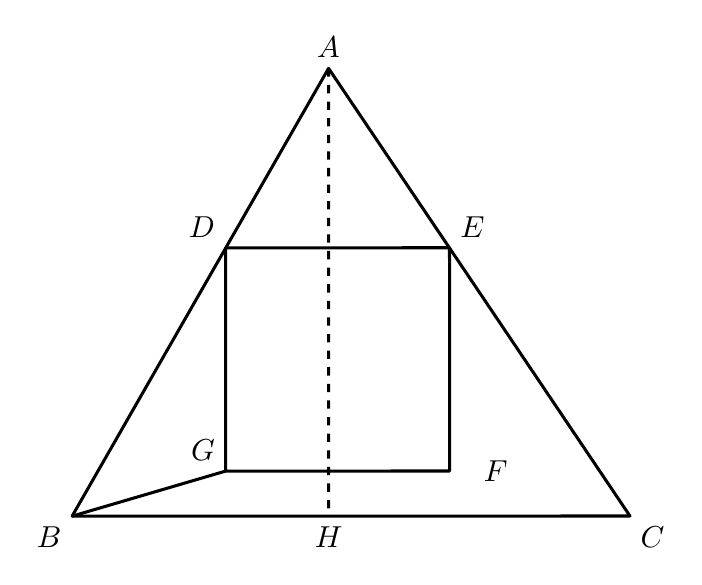
\begin{tikzpicture}[line join=round, line width=1.1pt, font=\fontsize{11}{13.2}\selectfont]

% Named coordinates (converted from pixels, s = 0.010025 cm/px, bbox centre (474,397))
\coordinate (A) at (-0.2851436593326893,2.8379136845288726);
\coordinate (B) at (-3.5416882501924536,-2.8490236399751456);
\coordinate (C) at (3.5424757829684097,-2.8472660965719676);
\coordinate (D) at (-1.5926138687094664,0.5587032308429625);
\coordinate (E) at (1.250905146867707,0.5594086927809194);
\coordinate (F) at (1.2516085465167281,-2.275797815077741);
\coordinate (G) at (-1.5919104690604453,-2.2765032770156983);
\coordinate (H) at (-0.2837332290577902,-2.847134779512202);

% Solid triangle ABC
\draw (A) -- (B) -- (C) -- cycle;

% Solid square DEFG
\draw (D) -- (E) -- (F) -- (G) -- cycle;

% Solid segment BG
\draw (B) -- (G);

% Dashed altitude AH
\draw[dashed] (A) -- (H);

% Labels
\node[above] at (A) {$A$};
\node[below left] at (B) {$B$};
\node[below right] at (C) {$C$};
\node[above left] at (D) {$D$};
\node[above right] at (E) {$E$};
% F label: right of vertex F, same height, 0.3 cm offset (no calc library needed)
\node[anchor=west] at ([xshift=0.3cm]F) {$F$};
\node[above left] at (G) {$G$};
\node[below] at (H) {$H$};

\end{tikzpicture}
\end{document}